%% if you are submitting an initial manuscript then you should have submission as an option here
%% if you are submitting a revised manuscript then you should have revision as an option here
%% otherwise options taken by the article class will be accepted
\documentclass[submission]{FPSAC2019}
%% but DO NOT pass any options (or change anything else anywhere) which alters page size / layout / font size etc

%% note that the class file already loads {amsmath, amsthm, amssymb}

\newtheorem{theorem}{Theorem}
\newtheorem{lemma}[theorem]{Lemma}
\newtheorem{proposition}[theorem]{Proposition}
\newtheorem{definition}[theorem]{Definition}
\newtheorem{example}[theorem]{Example}
\newtheorem{corollary}[theorem]{Corollary}
\newtheorem{conjecture}[theorem]{Conjecture}
\newtheorem{remark}[theorem]{Remark}
\newtheorem{notation}[theorem]{Notation}
\newtheorem{convention}[theorem]{Convention}
\newtheorem*{theorem*}{Theorem}%[section]

\usepackage{paralist}
\usepackage{xargs}
\usepackage{ulem}\normalem
\usepackage{pifont}
\usepackage{picins/picins}
\usepackage{tikz}
\usepackage{tkz-graph}
\usetikzlibrary{trees, decorations, decorations.markings, shapes, arrows, matrix, calc, fit, intersections, patterns, angles}

\graphicspath{{figures/}}

%%%%% AUTHOR'S COMMANDS %%%%%

% special letters
\newcommand{\R}{\mathbb{R}} % reals
\newcommand{\N}{\mathbb{N}} % naturals
\newcommand{\Z}{\mathbb{Z}} % integers
\newcommand{\C}{\mathbb{C}} % complex

% math commands
\newcommand{\set}[2]{\left\{ #1 \;\middle|\; #2 \right\}} % set notation
\newcommand{\bigset}[2]{\big\{ #1 \;|\; #2 \big\}} % big set notation
\newcommand{\biggset}[2]{\bigg\{ #1 \;\bigg|\; #2 \bigg\}} % bigg set notation
\newcommand{\ssm}{\smallsetminus} % small set minus
\newcommand{\dotprod}[2]{\langle \, #1 \; | \; #2 \, \rangle} % dot product
\newcommand{\symdif}{\,\triangle\,} % symmetric difference
\newcommand{\one}{{1\!\!1}} % the all one vector
\newcommand{\eqdef}{\mbox{\,\raisebox{0.2ex}{\scriptsize\ensuremath{\mathrm:}}\ensuremath{=}\,}} % :=
\newcommand{\defeq}{\mbox{~\ensuremath{=}\raisebox{0.2ex}{\scriptsize\ensuremath{\mathrm:}} }} % =:

% others
\newcommand{\ie}{\textit{i.e.}~} % id est
\newcommand{\eg}{\textit{e.g.}~} % exempli gratia
\newcommand{\Eg}{\textit{E.g.}~} % Exempli gratia
\newcommand{\viceversa}{\textit{vice versa}} % exempli gratia
\newcommand{\red}{\color{red}} % red command
\newcommand{\blue}{\color{blue}} % blue command
\definecolor{green}{RGB}{57,181,74} % green color
\newcommand{\green}{\color{green}} % green command
\newcommand{\defn}[1]{\uline{\textit{#1}}} % emphasis of a definition
\newcommand{\fref}[1]{Fig.\,\ref{#1}} % reference to figure

% COMBINATORICS
% quiver
\newcommand{\blossom}{^\text{\ding{96}}} % blossom
\newcommand{\Enrs}[1]{E_{nr}^{s}(#1)}
\newcommand{\Ers}[1]{E_{r}^{s}(#1)}
\newcommand{\Enrt}[1]{E_{nr}^{t}(#1)}
\newcommand{\Ert}[1]{E_{r}^{t}(#1)}

% walks
\newcommand{\peaks}[1]{\mathsf{peaks}(#1)} % peaks
\newcommand{\deeps}[1]{\mathsf{deeps}(#1)} % deeps
\newcommand{\distinguishedWalk}[2]{\mathsf{dw}(#1,#2)} % distinguished walk
\newcommand{\distinguishedArrows}[2]{\mathsf{da}(#1,#2)} % distinguished arrows
\newcommand{\distinguishedString}[2]{\mathsf{ds}(#1,#2)} % distinguished string
\newcommand{\distinguishedSign}[2]{\varepsilon(#1,#2)} % distinguished sign

% non-kissing complex, lattice, flip graph
\newcommand{\kn}{\kappa} % kissing number
\newcommand{\KN}{\textsc{kn}} % Kissing Number
\newcommandx{\NKC}[1][1=\bar Q]{\mathcal{K}_{\mathrm{nk}}(#1)} % non-kissing complex
\newcommandx{\RNKC}[1][1=\bar Q]{\mathcal{C}_{\mathrm{nk}}(#1)} % non-kissing complex
\newcommandx{\NKL}[1][1=\bar Q]{\mathcal{L}_{\mathrm{nk}}(#1)} % non-kissing lattice
\newcommandx{\NKG}[1][1=\bar Q]{\mathcal{G}_{\mathrm{nk}}(#1)} % non-kissing flip graph
\newcommandx{\NFC}[1][1=\bar Q]{\mathcal{C}_{\mathrm{nf}}(#1)} % non-friendly complex
\newcommand{\peak}{\mathrm{peak}} % bottom dissection
\newcommand{\deep}{\mathrm{deep}} % top dissection
\newcommand{\reversed}[1]{#1^{\mathrm{rev}}} % reverse all arrows
\renewcommand{\top}{\mathrm{top}} % top
\newcommand{\bottom}{\mathrm{bot}} % bottom
\newcommand{\walk}{\omega} % walk (of a curve)

% accordion and slalom complexes
\newcommand{\surface}{\mathcal{S}} % an orientable surface
\newcommand{\dual}{^*} % duality
\newcommand{\dissection}{\mathrm{D}} % dissection of a marked surface
\newcommand{\vertices}{\mathcal{V}} % vertices of a dissection
\newcommand{\edges}{\mathcal{E}} % edges of a dissection
\newcommand{\faces}{\mathcal{F}} % faces of a dissection
\newcommandx{\AC}[1][1=\dissection]{\mathcal{K}_{\mathrm{acc}}(#1)} % accordion complex
\newcommandx{\RAC}[1][1=\dissection]{\mathcal{C}_{\mathrm{acc}}(#1)} % reduced accordion complex
\newcommandx{\SC}[1][1=\dissection\dual]{\mathcal{K}_{\mathrm{sla}}(#1)} % slalom complex
\newcommandx{\RSC}[1][1=\dissection\dual]{\mathcal{C}_{\mathrm{sla}}(#1)} % reduced slalom complex
\newcommandx{\NCC}[1][1={\dissection, \dissection\dual}]{\mathcal{K}_{\mathrm{nc}}(#1)} % non-crossing complex
\newcommandx{\RNCC}[1][1={\dissection, \dissection\dual}]{\mathcal{C}_{\mathrm{nc}}(#1)} % non-crossing complex
\newcommand{\curveof}{\gamma} % curve (of a walk)
\newcommand{\edgeof}{\varepsilon} % arc of a vertex
\newcommand{\dualedgeof}{\varepsilon\dual} % dual arc of a vertex
\DeclareRobustCommand{\SSS}{\reflectbox{$\mathsf{Z}$}} % S
\DeclareRobustCommand{\ZZZ}{\mathsf{Z}} % Z
\newcommand{\koszul}{^!} % duality

%%%%% END AUTHOR'S COMMANDS %%%%%

%% define your title in the usual way
\title{Non-kissing versus non-crossing}

%% define your authors in the usual way
%% use \addressmark{1}, \addressmark{2} etc for the institutions, and use \thanks{} for contact details
\author{
	Yann Palu\thanks{\href{mailto:yann.palu@u-picardie.fr}{yann.palu@u-picardie.fr}. Supp. by ANR SC3A~15\,CE40\,0004\,01.}\addressmark{1},
	\stepcounter{footnote}
	Vincent Pilaud\thanks{\href{mailto:vincent.pilaud@lix.polytechnique.fr}{vincent.pilaud@lix.polytechnique.fr}. Supp. by ANR SC3A~15\,CE40\,0004\,01 and CAPPS~17\,CE40\,0018.}\addressmark{2},
	\and
	Pierre-Guy Plamondon\thanks{\href{mailto:pierre-guy.plamondon@math.u-psud.fr}{pierre-guy.plamondon@math.u-psud.fr}. Supp. by ANR SC3A~15\,CE40\,0004\,01 and a PEPS JCJC.}\addressmark{3}
}

%% then use \addressmark to match authors to institutions here
\address{
	\addressmark{1} LAMFA, Universit\'e Picardie Jules Verne, Amiens \\
	\addressmark{2} CNRS \& LIX, \'Ecole Polytechnique, Palaiseau, France \\
	\addressmark{3} Laboratoire de Math\'ematiques d'Orsay, Universit\'e Paris-Sud, CNRS, Universit\'e Paris-Saclay
}

%% put the date of submission here
\received{\today}

%% leave this blank until submitting a revised version
%\revised{}

%% put your English abstract here, or comment this out if you don't have one yet
%% please don't use custom commands in your abstract / resume, as these will be displayed online
%% likewise for citations -- please don't use \cite, and instead write out your citation as something like (author year)
\abstract{
Starting from a locally gentle bound quiver, we define on the one hand a simplicial complex, called the non-kissing complex.
On the other hand, we construct a punctured, marked, oriented surface with boundary, endowed with a pair of dual dissections.
From those geometric data, we define two simplicial complexes: the accordion complex, and the slalom complex, generalizing work of A.~Garver and T.~McConville in the case of a disk.
We show that all three complexes are isomorphic.
%, and that they are pure and thin.
%In particular, there is a notion of mutation on their facets, akin to $\tau$-tilting mutation.
%Along the way, we also construct inverse bijections between the set of isomorphism classes of locally gentle bound quivers and the set of homeomorphism classes of punctured, marked, oriented surfaces with boundary, endowed with a pair of dual dissections.
}

%% put your French abstract here, or comment this out if you don't have one
\resumetitle{R�sum�}
\resume{
�tant donn� un carquois localement aimable, nous d�finissons d'une part un complexe simplicial appel� complexe platonique. D'autre part, nous construisons une surface orientable � bord point�e et marqu�e, munie d'une paire de dissections duales. � partir de cette donn�e g�om�trique, nous d�finissons deux autres complexes simpliciaux : le complexe d'accord�ons et le complexe des slaloms qui g�n�ralisent les travaux de A.~Garver et T.~McConville dans le cas du disque. Nous montrons que ces trois complexes sont isomorphes.
}

%% put your keywords here, or comment this out if you don't have them yet
\keywords{Gentle algebras, non-kissing complex, non-crossing complex}

%% you can include your bibliography however you want, but using an external .bib file is STRONGLY RECOMMENDED and will make the editor's life much easier
%% regardless of how you do it, please use numerical citations, ie. [xx, yy] in the text

%% this sample uses biblatex, which (among other things) takes care of URLs in a more flexible way than bibtex
%% but you can use bibtex if you want
\usepackage[backend=bibtex, firstinits=true, maxbibnames=99]{biblatex}
\DeclareFieldFormat[article,inbook,incollection,inproceedings,patent,thesis,unpublished]{title}{\textit{#1}\isdot}
\renewbibmacro{in:}{}
\addbibresource{nonkissing-noncrossing-FPSAC.bib}
%% note the \printbibliography command at the end of the file which goes with these biblatex commands

\begin{document}

\maketitle
%% note that you DO NOT have to put your abstract here -- it is generated by \maketitle and the \abstract and \resume commands above

\section{Introduction}

This extended abstract reports on~\cite{PaluPilaudPlamondon-surfaces}, where more details and proofs are available.~It shows that two combinatorial objects, the \emph{non-kissing complex} and the \mbox{\emph{non-crossing complex}}, are isomorphic.
Both complexes appeared in different works in specific cases: the non-kissing complex of a grid appeared in \cite{McConville}, while the non-crossing complex of a disk appeared in \cite{GarverMcConville, MannevillePilaud-accordion}.
It was shown in \cite{PaluPilaudPlamondon} that these complexes are special cases of a more general simplicial complex, defined for any gentle algebra (see~also~\cite{BrustleDouvilleMousavandThomasYildirim}).

In order to unify these two objects, we are led to introduce two generalizations.
On the algebraic side, the non-kissing complex is extended from the class of gentle algebras to that of locally gentle algebras (which are an infinite-dimensional version of gentle algebras).
On the geometric side, we construct the non-crossing complex of an arbitrary oriented punctured surface endowed with a pair of dual dissections.

The two main objects of our study will thus be locally gentle algebras and dissections of surfaces.
Our first result is that these two classes of objects are essentially the~same.

\begin{theorem*}[see Thm.~\ref{thm:bijectionLocallyGentleAndSurfaces}]
There is an explicit bijection between the set of isomorphism classes of locally gentle bound quivers and the set of homeomorphism classes of oriented punctured marked surfaces with boundary endowed with a pair of dual cellular dissections.
\end{theorem*}

On the algebraic side, we extend the study of walks from the gentle case~\cite{McConville, PaluPilaudPlamondon} to the locally gentle case, and define a notion of compatibility called non-kissing (see Sect.\,\ref{sec:nonKissingComplex}).
On the geometric side, we extend the study of dissections, accordions and slaloms from the case of the disk~\cite{GarverMcConville, MannevillePilaud-accordion} to the case of an arbitrary surface, and define a notion of compatibility called non-crossing (see Sect.\,\ref{sec:accordionSlalomNonCrossingComplexes}).
The combinatorial information contained in these notions is encoded in simplicial complexes: the non-kissing complex~$\NKC$ and the non-crossing complex~$\NCC$.
Our second result is the following.

\begin{theorem*}[see Thm.~\ref{thm:complexesCoincide}]
The complexes~$\NKC$ and~$\NCC$ are isomorphic.
\end{theorem*}

%Finally, we show in Section \ref{sec:propertiesOfComplexes} that these complexes are combinatorially very well-behaved.
%
%\begin{theorem}[\ref{prop:purity} and \ref{coro:thin}]
%The complexes~$\NKC$ and~$\NCC$ are pure and thin.  Their dimension is computed, and mutation is explicitly described.
%\end{theorem}
%
%We end in Section \ref{sec:vectors} with a discussion of~$\b{g}$-vectors,~$\b{c}$-vectors and~$\b{d}$-vectors associated to walks and curves.
%Consequences on the representation theory of locally gentle algebras will be investigated in a future project.

Let us briefly review the algebraic and geometric objects which appear in this paper.
%
Gentle algebras are a class of finite-dimensional associative algebras over a field, defined by generators and relations.
Their representation theory was first systematically investigated in~\cite{ButlerRingel}, and they have been thouroughly studied since.
Locally gentle algebras are obtained by dropping the requirement that gentle algebras be finite-dimensional.
It turns out that their representation theory is also well-behaved \cite{Crawley-Boevey} and that these algebras are Koszul \cite{BessenrodtHolm}.
The $\tau$-tilting theory \cite{AdachiIyamaReiten} of gentle algebras was recently studied~in~\mbox{\cite{PaluPilaudPlamondon, BrustleDouvilleMousavandThomasYildirim}}.

Dissections of surfaces, on the other hand, are certain collections of pairwise non-intersecting curves on an orientable surface.
They have been defined and studied in \cite{Chapoton-quadrangulations, GarverMcConville, MannevillePilaud-accordion} in the case where the surface is an unpunctured disk.

The idea of associating a finite-dimensional algebra to a dissection (or a triangulation) of a surface seems to take its roots in the theory of cluster algebras and cluster categories.
This was first done for triangulations of polygons in \cite{CalderoChapotonSchiffler}, and then for any orientable surface with boundary in \cite{ABCP}.  
The algebra of a dissection as we shall use it in this paper has appeared in \cite{DavidRoeslerSchiffler}.
In most of the above cases, the algebras obtained are gentle algebras.
It has also been shown in \cite{BaurCoelhoSimoes} that any gentle algebra is obtained from a dissection of a surface, and that the module category of the algebra can be interpreted by using curves on the surface.
In the case where the surface is a polygon, the $\tau$-tilting theory of the algebra of a dissection has been studied in \cite{PaluPilaudPlamondon}.%, PilaudPlamondonStella}.

Conversely, the construction of a surface associated to a gentle algebra has appeared in \cite{OpperPlamondonSchroll}.
We give a different construction of the same surface in this paper, which is obtained by ``glueing'' quadrilaterals to the arrows of the blossoming quiver (as defined in \cite{PaluPilaudPlamondon}, and called ``fringed quiver'' in \cite{BrustleDouvilleMousavandThomasYildirim}).
Our construction has the advantage that it easily yields the two dual dissections of the surface at the same time (the dissection and dual lamination of \cite{OpperPlamondonSchroll}).
Note that our dissections are always cellular, while those in \cite{BaurCoelhoSimoes} can be arbitrary.
%Remarkably, gentle algebras and surfaces were linked recently in \cite{HaidenKatzarkovKontsevich, LekiliPolishchuk}, where the Fukaya category of the surface is shown to be equivalent to the bounded derived category of the associated gentle~algebra.

\section{Non-kissing complex}
\label{sec:nonKissingComplex}

%We first quickly review the definition of the non-kissing complex of a gentle bound quiver following the presentation of~\cite{PaluPilaudPlamondon} and extend it to locally gentle bound quivers.

\subsection{Locally gentle bound quivers and their blossoming quivers}

We consider a \defn{bound quiver}~$\bar Q = (Q,I)$, formed by a finite quiver~$Q = (Q_0, Q_1, s, t)$ and an ideal~$I$ of the path algebra~$kQ$ (the~$k$-vector space generated by all paths in~$Q$, including vertices as paths of length zero, with multiplication induced by concatenation of paths) such that~$I$ is generated by linear combinations of paths of length at least two.
Note that we \textbf{do not require} that the quotient algebra~$kQ/I$ be finite dimensional.
The following definition is adapted from~\cite{ButlerRingel}. We note that it is customary to consider non-finite dimensional gentle algebras in the literature, see e.g.~\cite{Schroer}.

\begin{definition}
\label{def:gentleQuiver}
A \defn{locally gentle bound quiver}~$\bar Q \eqdef (Q,I)$ is a (finite) bound quiver~where
\begin{compactenum}[(i)]
\item each vertex~$a \in Q_0$ has at most two incoming and two outgoing arrows,
\item the ideal~$I$ is generated by paths of length exactly two,
\item for any arrow~$\beta \in Q_1$, there is at most one arrow~$\alpha \in Q_1$ with~$t(\alpha) = s(\beta)$ and~${\alpha\beta\notin I}$ (resp.~$\alpha\beta \in I$) and at most one arrow~$\gamma \in Q_1$ with~$t(\beta) = s(\gamma)$~and~${\beta\gamma\notin I}$~(resp.~${\beta\gamma \in I}$).
\end{compactenum}
The algebra~$kQ/I$ is called a \defn{locally gentle algebra}.
A \defn{gentle bound quiver} is a locally gentle bound quiver~$\bar Q$ such that the algebra $kQ/I$ is finite-dimensional; $kQ/I$ is then a \defn{gentle algebra}.
\end{definition}

\begin{definition}
\label{def:blossomingQuiver}
A locally gentle bound quiver~$\bar Q$ is \defn{complete} if any vertex~$a \in Q_0$ is incident to either one ($a$ is a leaf) or four arrows ($a$ is an internal vertex).
The \defn{pruned subquiver} of a quiver~$\bar Q$ is the locally gentle quiver obtained by deleting all leaves of~$\bar Q$ (degree one vertices) and their incident arrows.
The \defn{blossoming quiver} of a locally gentle bound quiver~$\bar Q$ is the complete locally gentle bound quiver~$\bar Q\blossom$ whose pruned subquiver is~$\bar Q$.
The vertices of~$Q\blossom_0 \ssm Q_0$ are called \defn{blossom vertices}, and the arrows in~$Q\blossom_1 \ssm Q_1$ are called \defn{blossom arrows}. See \fref{fig:quivers}.
%
\begin{figure}[b]
	\centerline{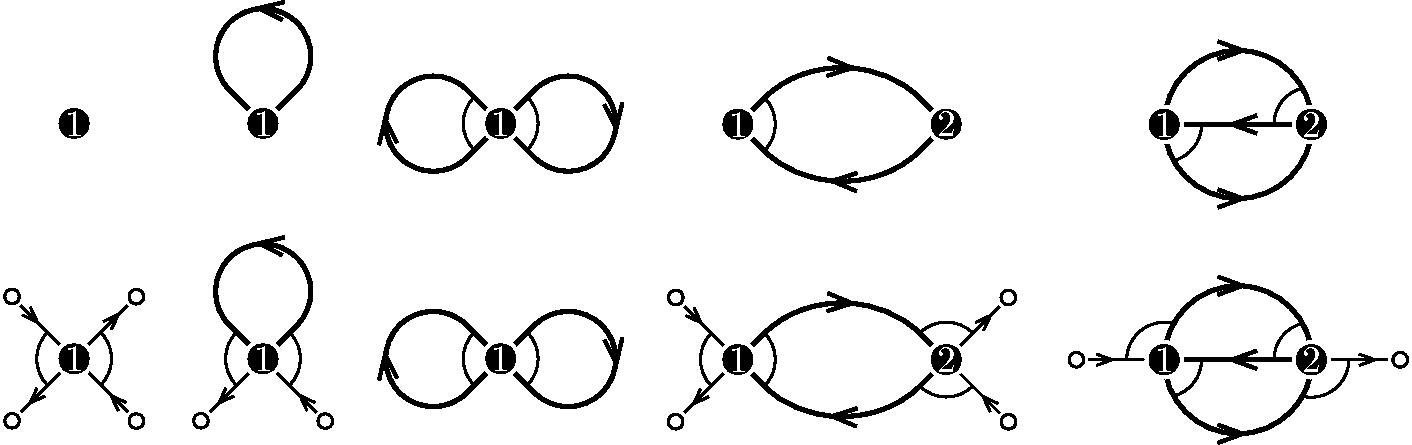
\includegraphics[scale=.6]{quivers}}
	\caption{Some locally gentle quivers (top) and their blossoming quivers (bottom).} %Initial vertices are solid and labeled while blossom vertices are hollow, and initial arrows are bold while blossom arrows are thin.}
	\label{fig:quivers}
\end{figure}
\end{definition}

%In other words, $\bar Q\blossom$ is obtained from~$\bar Q$ by adding blossom arrows and blossom vertices at each incomplete vertex of~$\bar Q$ and by completing~$I$ accordingly.
%Examples are represented on \fref{fig:quivers}.

\begin{remark}
\label{rem:sizeBlossomingQuiver}
Note that~$\bar Q\blossom$ has~$2|Q_0|-|Q_1|$ incoming blossom arrows and~$2|Q_0|-|Q_1|$ outgoing blossom arrows.
Therefore, it has $|Q_0\blossom| = |Q_0| + 2(2|Q_0|-|Q_1|) = 5|Q_0|-2|Q_1|$ vertices and~${|Q_1\blossom| = |Q_1| + 2(2|Q_0|-|Q_1|) = 4|Q_0|-|Q_1|}$ arrows.
\end{remark}

\subsection{Strings and walks}

The non-kissing complex is constructed using the combinatorics of strings and walks in the quiver~$\bar Q$, whose definitions are now briefly recalled.
The terminology and notations in the following definitions is borrowed from~\cite{ButlerRingel, Crawley-Boevey}.

For any arrow~$\alpha$ of~$Q$, define a formal inverse~$\alpha^{-1}$ with the properties that~${s(\alpha^{-1}) = t(\alpha)}$, $t(\alpha^{-1}) = s(\alpha)$, $\alpha^{-1}\alpha = \varepsilon_{t(\alpha)}$ and~$\alpha\alpha^{-1} = \varepsilon_{s(\alpha)}$, where~$\varepsilon_v$ is the path of length zero starting and ending at the vertex~$v \in Q_0$.

\begin{definition}
\label{def:string}
Let~$\bar Q = (Q,I)$ be a locally gentle bound quiver.
A \defn{finite string} in~$\bar Q$ is a word of the form
\(
\rho = \alpha_1^{\varepsilon_1}\alpha_2^{\varepsilon_2}\cdots \alpha_\ell^{\varepsilon_\ell},
\)
where
	\begin{compactenum}[(i)]
	\item $\alpha_i \in Q_1$ and~$\varepsilon_i \in \{-1,1\}$ for all~$i \in [\ell]$,
	\item $t(\alpha_i^{\varepsilon_i}) = s(\alpha_{i+1}^{\varepsilon_{i+1}})$ for all~$i \in [\ell-1]$,
	\item there is no path~$\pi \in I$ such that~$\pi$ or~$\pi^{-1}$ appears as a factor of~$\rho$, and
	\item $\rho$ is reduced, in the sense that no factor~$\alpha\alpha^{-1}$ or~$\alpha^{-1}\alpha$ appears in~$\rho$, for~$\alpha \in Q_1$.
	\end{compactenum}
The integer~$\ell$ is called the \defn{length} of the string~$\rho$.
We let~$s(\rho) \eqdef s(\alpha_1^{\varepsilon_1})$ and~$t(\rho) \eqdef t(\alpha_\ell^{\varepsilon_\ell})$ denote the source and target of~$\rho$.
For each vertex~$a \in Q_0$, there is also a \defn{string of length zero}, denoted by~$\varepsilon_a$, that starts and ends at~$a$.
\end{definition}

%\begin{example}
%With our choice of conventions, we represent the string ${\gamma\beta^{-1}\alpha^{-1}\gamma\beta^{-1}\alpha^{-1}\gamma\delta}$ by
%\[
%\;\vcenter{\hbox{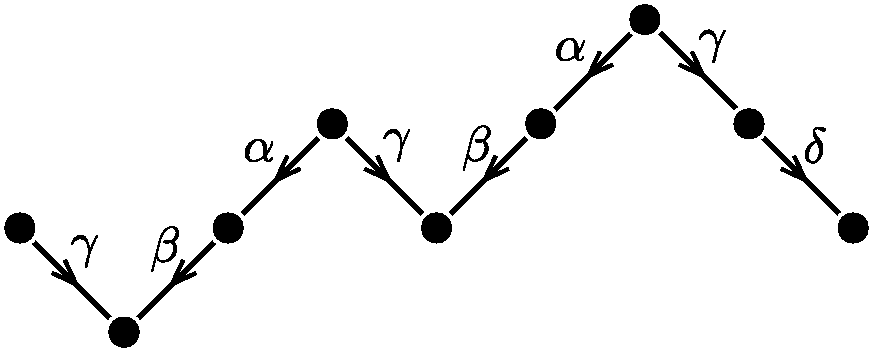
\includegraphics[scale=0.3]{exmString1}}}
%\]
%\end{example}

%\begin{definition}
%An oriented cycle~$c$ in~$Q$ such that~$c, c^2 \notin I$ is called \defn{primitive} if it cannot be written as an $n$-th power ($n>1$) of a cycle.
%\end{definition}

If~$c$ is an oriented cycle in~$Q$ such that~$c, c^2 \notin I$, we write $c^\infty$ for the infinite word~$c c c\cdots$, ${}^\infty c$ for the infinite word~$\cdots c c c$, and $^\infty c^\infty$ for the bi-infinite word~$^\infty c c^\infty$.
We also define~${}^{-\infty}c \eqdef {}^{\infty}(c^{-1}) = (c^\infty)^{-1}$ and similarly~$c^{-\infty} \eqdef (c^{-1})^\infty = (^\infty c)^{-1}$.

\begin{definition}
An \defn{eventually cyclic string} for~$\bar Q$ is a word~$\rho$ of the form~${}^\infty(c_1^{\varepsilon_1})\sigma (c_2^{\varepsilon_2})^\infty$, where $c_1, c_2$ are oriented cycles in~$\bar Q$ (possibly of length zero) and $\varepsilon_1, \varepsilon_2$ are signs in~$\{\pm 1\}$ such that $c_1^{2\varepsilon_1} \sigma c_2^{2\varepsilon_2}$ is a finite string in~$\bar Q$.
\end{definition}

\begin{definition}
A \defn{string} for~$\bar Q$ is a word which is either a finite string or an eventually cyclic infinite string.
We often implicitly identify the strings~$\rho$ and~$\rho^{-1}$, and call it an \defn{undirected string}.
\end{definition}

To avoid distinguishing between finite and (bi-)infinite words, we denote strings as pro\-ducts~$\rho = \prod_{i < \ell < j} \alpha_\ell^{\varepsilon_\ell}$ where~$i < j \in \Z \cup \{\pm \infty\}$, $\varepsilon_\ell\in\{\pm 1\}$ and~$\alpha_\ell \in Q_1$~for~all~${i < \ell < j}$.

\begin{definition}
\label{def:walk}
A \defn{walk} of a locally gentle quiver~$\bar Q$ is a maximal string of its blossoming quiver~$\bar Q \blossom$ (meaning that at each end it either reaches a blossom vertex of~$\bar Q \blossom$ or enters an infinite oriented cycle).
We implicitly identify the walks~$\omega$ and~$\omega^{-1}$, and call it an \defn{undirected walk}.
\end{definition}

\begin{definition}
\label{def:substrings}
A \defn{substring} of a walk~$\omega = \prod_{i < \ell < j} \alpha_\ell^{\varepsilon_\ell}$ of~$\bar Q$ is a string~$\sigma = \prod_{i' < \ell < j'} \alpha_\ell^{\varepsilon_\ell}$ of~$\bar Q$ for some~$i \le i' < j' \le j$, where the inequality~$i \le i'$ (resp.~$j' \le j$) is strict when~$i \ne -\infty$ (resp.~$j \ne \infty$). In other words, $\sigma$ is a factor of~$\omega$ such that
\begin{compactitem}
\item the endpoints of~$\sigma$ are not allowed to be the possible blossom endpoints of~$\omega$,
\item the position of~$\sigma$ as a factor of~$\omega$ matters.
\end{compactitem}
Note that the string~$\varepsilon_a$ is a substring of~$\omega$ for each occurence of~$a$ as a vertex of~$\omega$.
We denote by~$\Sigma(\omega)$ the set of substrings of~$\omega$.
We use the same notation for undirected walks. % (of course, substrings of an undirected walk are undirected).
\end{definition}

\begin{definition}
\label{def:topBottom}
We say that the substring~$\sigma = \prod_{i' < \ell < j'} \alpha_\ell^{\varepsilon_\ell}$ is \defn{at the bottom} (resp.~\defn{on top}) of the walk~$\omega = \prod_{i < \ell < j} \alpha_\ell^{\varepsilon_\ell}$ if~$i'=-\infty$ or~$\varepsilon_{i'} = 1$ and~$j'=+\infty$ or~$\varepsilon_{j'} = -1$ (resp.~if~${i'=-\infty}$ or~${\varepsilon_{i'} = -1}$ and~$j'=\infty$ or~$\varepsilon_{j'} = 1$).
In other words the (at most) two arrows of~$\omega$ incident to the endpoints of~$\sigma$ point towards~$\sigma$ (resp.~outwards from~$\sigma$).
We denote by~$\Sigma_\bottom(\omega)$ and~$\Sigma_\top(\omega)$ the sets of bottom and top substrings of~$\omega$.
We use the same notations for undirected~walks.
\end{definition}

\begin{definition}
\label{def:straightBending}
%A \defn{peak} (resp.~\defn{deep}) of a walk~$\omega$ is a substring of~$\omega$ of length zero which is on top (resp.~at the bottom of~$\omega$).
%A \defn{corner} is either a peak or a deep (in other words, it is a vertex of~$\omega$ where the arrows change direction).
A walk~$\omega$ is \defn{straight} if~$\omega$ or~$\omega^{-1}$ is a path in~$\bar Q\blossom$, and \defn{bending} otherwise.
%A \defn{peak walk} (resp.~\defn{deep walk}) is a walk with a unique corner, which is a peak (resp.~deep). For~$a \in Q_0$, we denote by~$a_\peak$ the peak walk with peak at~$a$ and by~$a_\deep$ the deep walk with deep~at~$a$ (note that those are indeed unique by gentleness).
\end{definition}

\subsection{Non-kissing complex}

We can now define the non-kissing complex of a locally gentle bound quiver following~\cite{McConville, PaluPilaudPlamondon, BrustleDouvilleMousavandThomasYildirim}.
We start with the kissing relation for walks.

\parpic(5cm,2cm)(-2pt, 65pt)[r][b]{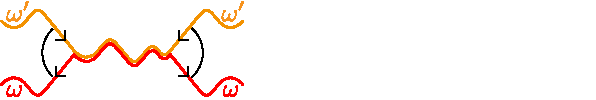
\includegraphics[scale=1.2]{kissing}}
\begin{definition}
\label{def:kiss}
Let~$\omega$ and~$\omega'$ be two undirected walks on~$\bar Q$.
We say that~$\omega$ \defn{kisses}~$\omega'$ if ${\Sigma_\top(\omega) \cap \Sigma_\bottom(\omega')}$ contains a \emph{finite} substring.
%See \fref{fig:kissing}.
We say that~$\omega$ and~$\omega'$ are \defn{kissing} if~$\omega$ kisses~$\omega'$ or~$\omega'$ kisses~$\omega$ (or both).
We allow the situation where the common finite substring is reduced to a vertex~$a$, meaning that~$a$ is a peak of~$\omega$ and a deep of~$\omega'$.
Note also that~$\omega$ can kiss~$\omega'$ several times, that~$\omega$ and~$\omega'$ can mutually kiss, and that~$\omega$ can kiss itself.
%
%\begin{figure}[h]
%	\centerline{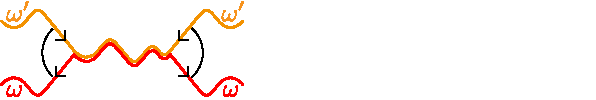
\includegraphics[scale=1]{kissing}}
%	\caption{A schematic representation of two kissing walks: $\omega$~kisses~$\omega'$.}
%	\label{fig:kissing}
%\end{figure}
%
\end{definition}

\begin{definition}
\label{def:nKc}
The \defn{non-kissing complex} of~$\bar Q$ is the simplicial complex~$\NKC$ whose faces are the sets of pairwise non-kissing walks of~$\bar Q$.
Note that self-kissing walks are excluded from the vertex set of this complex.
%Note that self-kissing walks never appear in~$\NKC$ by definition.
%In contrast, no straight walk can kiss another walk by definition, so that they appear in all facets of~$\NKC$.
%The \defn{reduced non-kissing complex}~$\RNKC$ is the simplicial complex whose faces are the collections of pairwise non-kissing bending walks of~$\bar Q$.
\end{definition}

\section{Accordions, slaloms, and non-crossing complex}\label{sec:accordionSlalomNonCrossingComplexes}

%We now temporarily switch topic and present the accordion complex and the slalom complex of a pair of dual dissections of an orientable surface.
%The latter is directly inspired from the case of a disk treated in~\cite{GarverMcConville}, while the former is obtained by duality as was already observed in the case of a disk in~\cite{MannevillePilaud-accordion}.
%In the general case of arbitrary orientable surfaces, the correspondence between accordions and slaloms requires a little more attention and is treated in Sect.~\ref{subsec:accordionsVSSlaloms}.

\subsection{Dual dissections of a surface}

Before defining accordions and slaloms, we need a strong notion of pairs of dual dissections of an orientable surface.
We first review classical definitions of curves, arcs and dissections of a surface adapting it to our setting.

\begin{definition}
A \defn{marked surface}~$\bar\surface \eqdef (\surface, M)$ is an orientable surface~$\surface$ with boundaries, together with a set~$M$ of marked points which can be on the boundary of~$\surface$ or not.
For~$V \subset \surface$,
\begin{compactenum}[(i)]
\item a \defn{$V$-arc} on~$\bar\surface$ is a curve on~$\surface$ connecting two points of~$V$ and whose interior is disjoint from~$M$ and the boundary of~$\surface$.
\item a \defn{$V$-curve} on~$\bar\surface$ is a curve on~$\surface$ which at each end either reaches a point of~$V$ or infinitely circles around and finally reaches a puncture of~$M$, and whose interior is disjoint from~$M$ and the boundary of~$\surface$.
\end{compactenum}
As usual, curves and arcs are considered up to homotopy relative to their endpoints in~$\surface \ssm M$, and curves homotopic to a boundary are not allowed.
\end{definition}

\begin{definition}
\label{def:crossingCurves}
Two curves or arcs \defn{cross} when they intersect in~their~interior.
We will always assume that collections of arcs on a surface are in minimal position, in the sense that they cross each other transversaly, and the number of crossings is minimal.
%It is pointed out in \cite{Thurston} that this assumption can always be satisfied (up to homotopy).
\end{definition}

\begin{definition}
A \defn{dissection} of~$\bar\surface$ is a collection~$\dissection$ of pairwise non-crossing arcs on~$\bar\surface$.
The \defn{edges} of~$\dissection$ are its arcs together with the boundary arcs of~$\bar\surface$.
The \defn{faces} of~$\dissection$ are the connected components of the complement of the union of the edges of~$\dissection$ in the surface~$\surface$.
We denote by~$\vertices(\dissection)$, $\edges(\dissection)$ and~$\faces(\dissection)$ the sets of vertices, edges and faces of~$\dissection$ respectively.
The dissection~$\dissection$ is \defn{cellular} if all its faces are topological disks.
For~$V \subseteq M$, a \defn{$V$-dissection} is a dissection with only $V$-arcs.
\end{definition}

\begin{convention}
\textbf{All throughout the paper, all dissections are considered cellular.}
\end{convention}

\begin{definition}
Consider a marked surface~$\bar\surface = (\surface, V \sqcup V\dual)$, where~$V$ and~$V\dual$ are two disjoint sets of marked points so that the points of~$V$ and~$V\dual$ that are on the boundary of~$\surface$ alternate.
A cellular $V$-dissection~$\dissection$ of~$\bar\surface$ and a cellular $V\dual$-dissection~$\dissection\dual$ of~$\bar\surface$ are \defn{dual cellular dissections} if there are pairs of mutually inverse bijections~$V\dual \leftrightarrow \faces(\dissection)$ and~$V \leftrightarrow \faces(\dissection\dual)$, both denoted~$\dual$ in both directions, such that~$\dissection$ has an edge joining its vertices~$u,v \in V$ and separating its faces~$f,g \in  \faces(\dissection)$ if and only if~$\dissection\dual$ has an edge joining its vertices~$f\dual, g\dual \in V\dual$ and separating its faces~$u\dual, v\dual \in \faces(\dissection\dual)$.
\end{definition}

Some examples of dual cellular dissections on different surfaces are represented in \fref{fig:dissections}.
%
\begin{figure}[t]
	\centerline{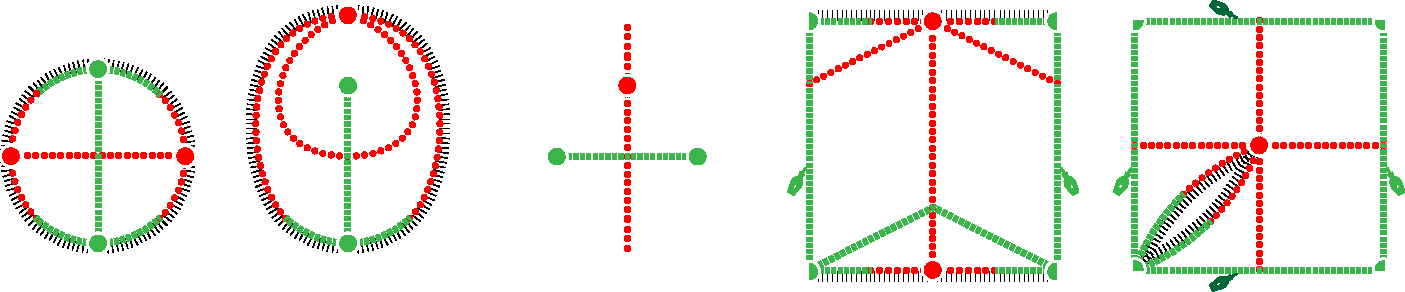
\includegraphics[scale=.7]{dissections}}
	\caption{Some pairs~$(\dissection, \dissection\dual)$ of dual cellular dissections on different surfaces. The dissection~$\dissection$ is in green while its dual dissection~$\dissection\dual$ is~in~red. The boundaries of the surfaces are shaded, and the glue symbols indicate how to identify edges.}
	\label{fig:dissections}
\end{figure}
%
Note that contrarily to the usual conventions, the dual vertex~$f\dual$ of a face~$f$ of~$\dissection$ is not always in the interior of the face~$f$.
More precisely, each face~$f$ has either no or exactly one edge on the boundary of~$\surface$. Its dual vertex~$f\dual$ then lies in the interior~of~$f$ and is a puncture of~$\bar\surface$ in the former case, and on the boundary edge of~$f$ in the latter~case.

%More precisely, there are two situations:
%\begin{compactitem}
%\item if a face~$f$ has no edges on the boundary of~$\surface$, its dual vertex~$f\dual$ lies in the interior~of~$f$ and is a puncture of~$\bar\surface$,
%\item if a face~$f$ has an edge on the boundary of~$\surface$, then it has exactly one such edge and its dual vertex~$f\dual$ lies on this edge.
%\end{compactitem}
%In fact, the second point forces the following characterization of the cellular dissections that admit a dual cellular dissection.
%
%\begin{proposition}
%\label{prop:conditionsDualDissections}
%For a cellular $V$-dissection~$\dissection$ of a marked surface~$\bar\surface = (\surface, V \sqcup V\dual)$, the following assertions are equivalent:
%\begin{compactenum}[(i)]
%\item there exists a cellular $V\dual$-dissection~$\dissection\dual$ of~$\bar\surface$ such that~$\dissection$ and~$\dissection\dual$ are dual cellular dissections,
%\item each face of~$\dissection$ contains exactly one point of~$V\dual$ (in particular, at most one boundary edge).
%\end{compactenum}
%Moreover, the cellular dissection~$\dissection\dual$ is uniquely determined.
%\end{proposition}
%
%\begin{proof}
%We mimick the proof of~\cite[Prop.~1.12]{OpperPlamondonSchroll}.
%The direct implication is immediate by definition.
%Assume conversely that each face~$f$ of~$\dissection$ contains exactly one point~$f\dual$ of~$V\dual$.
%We construct half-edges of~$\dissection\dual$ in each face~$f$ of~$\dissection$ by joining the dual point~$f\dual$ to the middle of each boundary edge of~$f$ that is not a boundary edge of~$\surface$.
%For each edge~$a$ of~$\dissection$, the half-edges incident to the middle of~$a$ in the two faces of~$\dissection$ containing~$a$ form the dual edge~$a\dual$ of~$a$.
%All these dual edges do not cross (as the half-edges do not cross in each face of~$\dissection$) and form the dual cellular dissection~$\dissection\dual$~of~$\dissection$.
%\end{proof}

\begin{definition}
We consider a set~$B$ of points on the boundary of the surface~$\surface$ such that~$B$ and~$V \cup V\dual$ alternate along the boundary of~$\surface$.
The points of~$B$ are called the \defn{blossom points}.
See \eg Figs.\,\ref{fig:accordions} \&~\ref{fig:slaloms} where the blossom points appear as white hollow vertices.
\end{definition}

\subsection{Accordion complex and slalom complex}

Let~$\bar\surface = (\surface, V \sqcup V\dual)$ be a surface with two disjoint sets~$V$ and~$V\dual$ of marked points, and let~$B$ be the corresponding blossom points on the boundary of~$\surface$.
%We say that a $B$-curve is \defn{external} if it is homotopic to a boundary arc of~$\surface \ssm B$, and \defn{internal} otherwise.
%Note that no $B$-curve can cross an external $B$-curve.
Consider two dual cellular dissections~$\dissection$ and~$\dissection\dual$ of~$\bar\surface$.
%
The next definition generalises the one of \cite{MannevillePilaud-accordion} for the case where~$\bar \surface$ is a disk. % A~very similar definition appears in \cite{BaurCoelhoSimoes} in a slightly different context under the \mbox{name ``permissible~arc''}.

\begin{definition}
\label{def:accordion}
A \defn{$\dissection$-accordion} is a $B$-curve~$\alpha$ of~$\bar\surface$ such that whenever~$\alpha$ meets a face~$f$~of~$\dissection$,
\begin{compactenum}[(i)]
\item it enters crossing an edge~$a$ of~$f$ and leaves crossing an edge~$b$ of~$f$ (in other words, $\alpha$ is not allowed to circle around~$f\dual$ when~$f\dual$ is a puncture),
\item the two edges~$a$ and~$b$ of~$f$ crossed by~$\alpha$ are consecutive along the boundary of~$f$,
\item $\alpha$, $a$ and~$b$ bound a disk inside~$f$ that does not contain~$f\dual{}$.
\end{compactenum}
By convention, we also consider that the punctures of~$V$ are $\dissection$-accordions.
%By convention, we also consider that the punctures of~$V$ are external $\dissection$-accordions.
%If we were working on the universal cover of the surface, the~$\dissection$-accordion associated to a puncture would be the infinite line crossing all (infinitely many) arcs attached to the puncture.
\end{definition}

\fref{fig:accordions} illustrates some $\dissection$-accordions for the dissections~$\dissection$ of \fref{fig:dissections}.

\begin{figure}[h]
	\centerline{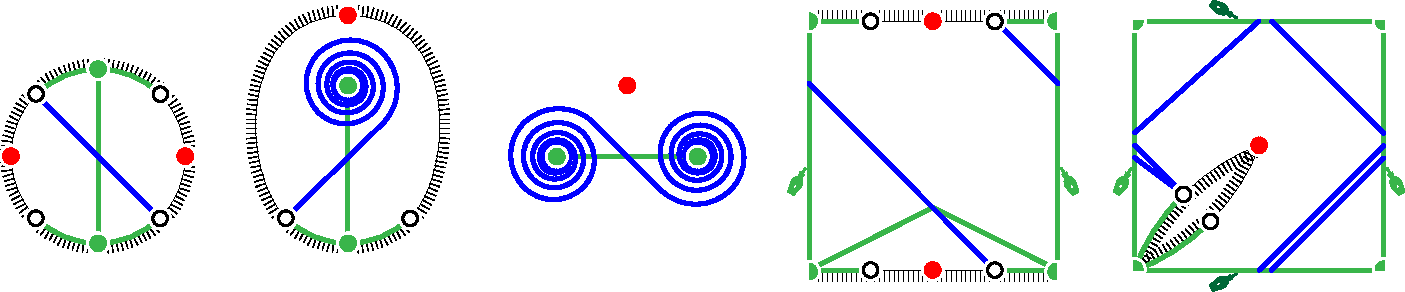
\includegraphics[scale=.7]{accordions}}
	\caption{Some $\dissection$-accordions (in blue) for the dissections~$\dissection$ of \fref{fig:dissections} (in green).}
	\label{fig:accordions}
\end{figure}

\begin{remark}
In Def.\,\ref{def:accordion}, observe that
\begin{compactitem}
\item the edges of~$a$ and~$b$ of~$f$ crossed by~$\alpha$ might coincide, see the second example in \fref{fig:accordions}.
\item the first condition is automatically satisfied if~$f\dual$ is not a puncture. %, \ie when it lies on the boundary of~$\surface$.
\end{compactitem}
\end{remark}

\begin{definition}
\label{def:accordionComplex}
The \defn{$\dissection$-accordion complex}~$\AC$ is the simplicial complex whose faces are the sets of pairwise non-crossing $\dissection$-accordions.
Note that self-crossing accordions are~excluded from the vertex set of this complex.
%Note that self-crossing accordions never appear in~$\AC$ by definition.
%In contrast, no external accordion can cross another accordion, so that they appear in all facets of~$\AC$. 
%The \defn{reduced $\dissection$-accordion complex}~$\RAC$ is the simplicial complex whose faces are the collections of pairwise non-crossing internal $\dissection$-accordions.
\end{definition}

The following definition generalizes the one from~\cite{GarverMcConville} for the case where~$\bar\surface$ is a disk.

\begin{definition}
\label{def:slalom}
A \defn{$\dissection\dual$-slalom} is a $B$-curve~$\alpha$ of~$\bar\surface$ such that, whenever~$\alpha$ crosses an edge~$a\dual$ of~$\dissection\dual$ contained in two faces~$f\dual, g\dual$ of~$\dissection\dual$, the marked points~$f$ and~$g$ lie on opposite sides of~$\alpha$ in the union of~$f\dual$ and~$g\dual$ glued along~$a\dual$.
Here, we consider that~$f$ lies on the right (resp.~left) of~$\alpha$ when~$\alpha$ circles clockwise (resp.~counterclockwise) around~$f$.
By convention, we also consider that the punctures of~$V$ are $\dissection\dual$-slaloms.
%By convention, we also consider that the punctures of~$V$ are external $\dissection\dual$-slaloms.
%If we were working on the universal cover of the surface, the~$\dissection\dual$-slalom associated to a puncture would be an infinite line never crossing any arc of~$\dissection\dual$.
\end{definition}

\fref{fig:slaloms} illustrates some $\dissection\dual$-slaloms for the dual dissections~$\dissection\dual$ of \fref{fig:dissections}.

\begin{figure}[h]
	\centerline{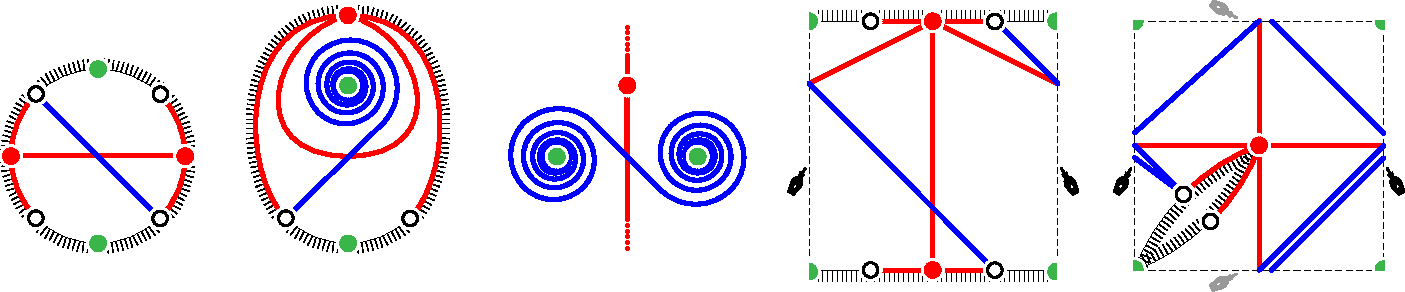
\includegraphics[scale=.7]{slaloms}}
	\caption{Some $\dissection\dual$-slaloms (in blue) for the dual dissections~$\dissection\dual$ of \fref{fig:dissections} (in red).}
	\label{fig:slaloms}
\end{figure}

\begin{definition}
\label{def:slalomComplex}
The \defn{$\dissection\dual$-slalom complex}~$\SC$ is the simplicial complex whose faces are the sets of pairwise non-crossing $\dissection\dual$-slaloms.
Note that self-crossing slaloms are forbidden.
%Note that self-crossing slaloms never appear in~$\SC$ by definition.
%In contrast, no external slalom can cross another slalom, so that they appear in all facets of~$\SC$. 
%The \defn{reduced $\dissection\dual$-slalom complex}~$\RSC$ is the simplicial complex whose faces are the collections of pairwise non-crossing internal $\dissection\dual$-slaloms.
\end{definition}

\subsection{Accordions versus slaloms and the non-crossing complex}
\label{subsec:accordionsVSSlaloms}

%The following statement is illustrated by Figures~\ref{fig:accordions} and~\ref{fig:slaloms}.

\begin{proposition}
\label{prop:accordionsSlaloms}
For two dual cellular dissections~$\dissection$ and~$\dissection\dual$, the $\dissection$-accordions are precisely the $\dissection\dual$-slaloms and the $\dissection$-accordion complex coincides with the $\dissection\dual$-slalom complex.
See Figs.\,\ref{fig:accordions} \& \ref{fig:slaloms}.
\end{proposition}

%\begin{proof}
%Let~$\alpha$ be a~$\dissection$-accordion.
%Let~$a$,~$b$,~$c$ be three consecutive edges of~$\dissection$ crossed by~$\alpha$.
%Let~$u \in \dissection$ be the common endpoint of~$a$ and $b$ given by Definition~\ref{def:accordion} and let~$v \in \dissection$ be the common endpoint of~$b$ and~$c$.
%If $u = v$, then the segment of~$\alpha$ between~$a$ and~$c$ stays in the same face of~$\dissection\dual$.
%Otherwise, when crossing~$b$, the accordion~$\alpha$ leaves the face~$u\dual$ of $\dissection\dual$ and enters the face~$v\dual$.
%In the surface obtained by glueing the two cells~$u\dual$ and~$v\dual$ along~$b\dual$, the marked points~$u$ and~$v$ are separated by~$\alpha$.
%Conversely, assume that~$\alpha$ is an curve of~$(\surface, B)$ which is not a $\dissection$-accordion.
%We are in one of the following cases.
%
%Case 1: The curve~$\alpha$ consecutively crosses two edges~$a$ and~$b$ of~$\dissection$ that do not share a common endpoint.
%Let~$f$ be the face of~$\dissection$ that contains the segment of~$\alpha$ between~$a$ and~$b$.
%Consider the connected component of~$f\setminus\alpha$ that does not contain~$f\dual$.
%The boundary of this component contains an edge~$c \in \dissection \setminus \{a\}$ that shares a common endpoint with~$a$.
%Let~$u,v$ be the endpoints~of~$c$.
%Then~$\alpha$ cuts the cells $u\dual,v\dual$ glued along~$c\dual$ into two connected components, one containing both~endpoints~of~$c$.
%
%Case 2: The curve~$\alpha$ consecutively crosses two edges~$a$ and~$b$ of~$\dissection$ that share a unique common endpoint, but the region delimited by~$\alpha$,~$a$ and~$b$ is not a disk.
%Since the dissection~$\dissection$ is cellular, that region has to contain some marked point~$u \in \dissection\dual$.
%One conclude that~$\alpha$ is not a~$\dissection\dual$-slalom similarly as in the first case, by considering the component of~$u\dual \setminus \alpha$ that does not contain~$u$.
%
%Case 3: The curve~$\alpha$ consecutively crosses two edges~$a$ and~$b$ of~$\dissection$ that share two different endpoints, and none of the two regions delimited by~$\alpha$,~$a$ and~$b$ is a disk.
%Since the dissection~$\dissection$ is cellular, both regions have to contain a puncture.
%This contradicts the assumption that the dissections~$\dissection$ and~$\dissection\dual$ are dual to each other.
%
%Case 4: If~$\alpha$ stays inside a $\dissection$-cell, then it rolls around a~$\dissection\dual$ puncture.
%There is a~$\dissection\dual$-edge~$a$ ending in that puncture. When~$\alpha$ crosses~$a$, the puncture stays on the same side of~$\alpha$, hence~$\alpha$ is not a~$\dissection\dual$-slalom.
%\end{proof}

\begin{definition}
\label{def:noncrossingComplex}
The \defn{non-crossing complex} of the pair of dual cellular dissections~$(\dissection, \dissection\dual)$ is the simplicial complex~$\NCC \eqdef \AC = \SC$.
%The \defn{reduced non-crossing complex} of~$(\dissection, \dissection\dual)$ is~$\RNCC \eqdef \RAC = \RSC$.
\end{definition}

%\begin{remark}
%The $\dissection$-slaloms and the $\dissection\dual$-accordions are defined dually and also coincide.
%\end{remark}

%\begin{example}
%When the dissection~$\dissection$ is a classical dissection of a polygon (with no punctures) where each cell has at most one boundary edge, the dual dissection~$\dissection\dual$ is a tree.
%The non-crossing complex in this situation was treated in detail in~\cite{GarverMcConville, MannevillePilaud-accordion}.
%Note that even when the surface~$\surface$ is a disk, we authorize in the present paper both~$\dissection$ and~$\dissection\dual$ to have interior faces and punctures.
%\end{example}

%\begin{remark}
%A quick disclaimer about accordion complexes and slalom complexes of arbitrary cellular dissections.
%As stated in Proposition~\ref{prop:conditionsDualDissections}, a cellular dissection~$\dissection$ with a face containing more than one boundary edge does not admit a dual cellular dissection~$\dissection\dual$.
%This prevents the use of the definitions given in this section.
%Although the accordion complex (resp.~slalom complex) could still be defined as in~\cite{MannevillePilaud-accordion} (resp.~\cite{GarverMcConville}) for the disk, the resulting complexes would be joins of smaller accordion complexes (resp.~slalom complexes) defined in this paper.
%See \cite[Prop.~2.4]{MannevillePilaud-accordion} for a detailed statement in the case of the disk.
%\end{remark}

\section{Non-kissing versus non-crossing}

%In this section, we show that non-kissing and non-crossing complexes actually coincide.
%Namely, any pair of dual cellular dissections~$(\dissection, \dissection\dual)$ defines a locally gentle bound quiver~$\bar Q_{\dissection}$ (see Section~\ref{subsec:D2Q}) such that the non-crossing complex~$\NCC$ is isomorphic to the non-kissing complex~$\NKC[\bar Q_{\dissection}]$.
%Conversely, any locally gentle bound quiver~$\bar Q$ gives rise to a surface~$\surface_{\bar Q}$ equipped with a pair of dual cellular dissections~$\dissection_{\bar Q}$ and~${{\dissection\dual}\!\!_{\bar Q}}$ (see Section~\ref{subsec:Q2D}) such that the non-kissing complex~$\NKC$ is isomorphic to the non-crossing complex~$\NCC[\dissection_{\bar Q}, {\dissection\dual\!\!_{\bar Q}}]$.
%In fact, we show that the accordion, slalom, and non-kissing complexes can all be pictured in a unique way on the surface.
%Interestingly, via the correspondence between pairs of dual cellular dissections and locally gentle bound quivers, the duality between the dissections~$\dissection$ and~$\dissection\dual$ translates into the Koszul duality between the locally gentle algebras of~$\bar Q$ and~$\bar Q\koszul$.
%Many examples are treated in Section~\ref{subsec:Q2D}.

\subsection{The bound quiver of a dissection}
\label{subsec:D2Q}

We first associate a quiver to a pair of dual dissections~$(\dissection,\dissection\dual)$.% of a marked surface~$(\surface, V\sqcup V\dual)$.
%Let~$\dissection$ and~$\dissection\dual$ be two dual cellular dissections of a marked surface~$(\surface, V\sqcup V\dual)$.
%Let $B$ be the set of blossom points.

\begin{definition}
\label{def:quiverDualDissections}
The quiver of the dissection~$\dissection$ is the quiver $\bar Q_{\dissection} = (Q_{\dissection}, I_{\dissection})$ defined~by:
\begin{compactenum}[(i)]
\item the set of vertices of~$Q_{\dissection}$ is the set of edges of $\dissection$;
\item there is an arrow from~$a$ to~$b$ for each common endpoint~$v$ of~$a$ and~$b$ such that~$b$ comes immediately after~$a$ in the counterclockwise order around~$v$;
\item the ideal~$I_{\dissection}$ is generated by the paths of length two in~$Q_{\dissection}$ obtained by composing arrows which correspond to triples of consecutive edges in a face of~$\dissection$.
\end{compactenum}
The bound quiver of the dissection~$\dissection\dual$ is the bound quiver $\bar Q_{\dissection\dual} = (Q_{\dissection\dual}, I_{\dissection\dual})$ defined by replacing~$\dissection$ by~$\dissection\dual$ in the above.
See \fref{fig:quiversDissections}.
%
\begin{figure}[h]
	\centerline{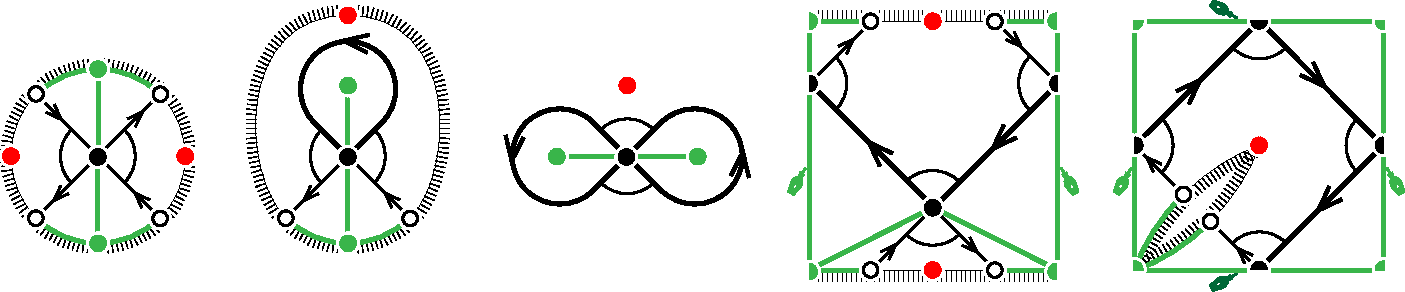
\includegraphics[scale=.7]{quiversDissections1}}
	\medskip
	\centerline{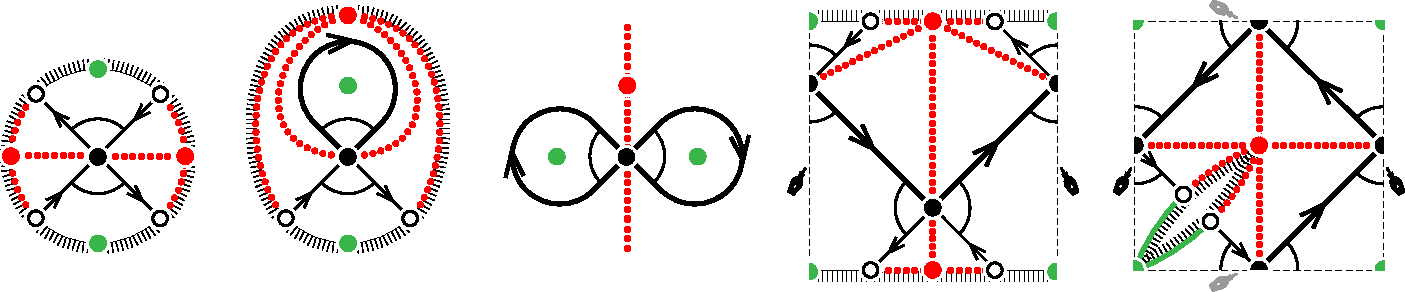
\includegraphics[scale=.7]{quiversDissections2}}
	\caption{The quivers associated to the dissections of \fref{fig:dissections}.}% As stated in Proposition~\ref{prop:dualityKoszul1}, dual dissections give rise to Koszul dual bound quivers.}
	\label{fig:quiversDissections}
\end{figure}
\end{definition}

%\fref{fig:quiversDissections} illustrates this construction for the dissections of \fref{fig:dissections}.

\begin{remark}
The blossoming quiver~$\bar Q_\dissection\blossom$ of the quiver~$\bar Q_\dissection$ is obtained with the same procedure by considering additional blossom vertices along the boundary of the surface. See \fref{fig:quiversDissections}.
\end{remark}

\begin{lemma}
\label{lemm:quiverOfDissectionIsLocallyGentle}
The bound quiver~$\bar Q_{\dissection} = (Q_{\dissection}, I_{\dissection})$ is a locally gentle bound quiver.
\end{lemma}

%\begin{proof}
%Each edge~$a$ of~$\dissection$ has two endpoints, and at each endpoint there is at most one edge of~$\dissection$ coming immediately after~$a$ in the clockwise order, and at most one edge of~$\dissection$ coming immediately before~$a$.
%Thus, in~$Q_{\dissection}$, there are at most two arrows leaving~$a$ and at most two arriving in~$a$.
%Among these arrows, those arising from the same endpoint of~$a$ will be composable, and those arising from different endpoints will yield relations.
%Thus $\bar Q_{\dissection}$ is locally gentle.
%\end{proof}

\begin{definition}
\label{defi:koszulDual}
The \defn{Koszul dual} of a locally gentle bound quiver~$\bar Q = (Q,I)$~is the bound quiver~$\bar Q\koszul = (Q\koszul, I\koszul)$ defined as follows:
\begin{compactenum}[(i)]
\item the quiver~$Q\koszul$ is equal to the opposite quiver of~$Q$ (obtained from~$Q$ by reversing all arrows);
\item the ideal~$I\koszul$ is generated by the opposites of the paths of length two in~$Q$ that are not in~$I$.
\end{compactenum}
\end{definition}

%It is seen in \cite{BessenrodtHolm} that the (ungraded version of the) Koszul dual of a locally gentle algebra~$kQ/I$ is isomorphic to~$kQ\koszul/I\koszul$.
%Note that~$\bar Q\koszul$ is locally gentle, and that Koszul duality is an involution and commutes with blossoming:~$(\bar Q\koszul)\koszul = \bar Q$ and~$(\bar Q\koszul)\blossom = (\bar Q\blossom)\koszul$.
%%Examples are represented on \fref{fig:koszulQuivers}.
%%
%%\begin{figure}[t]
%%	\centerline{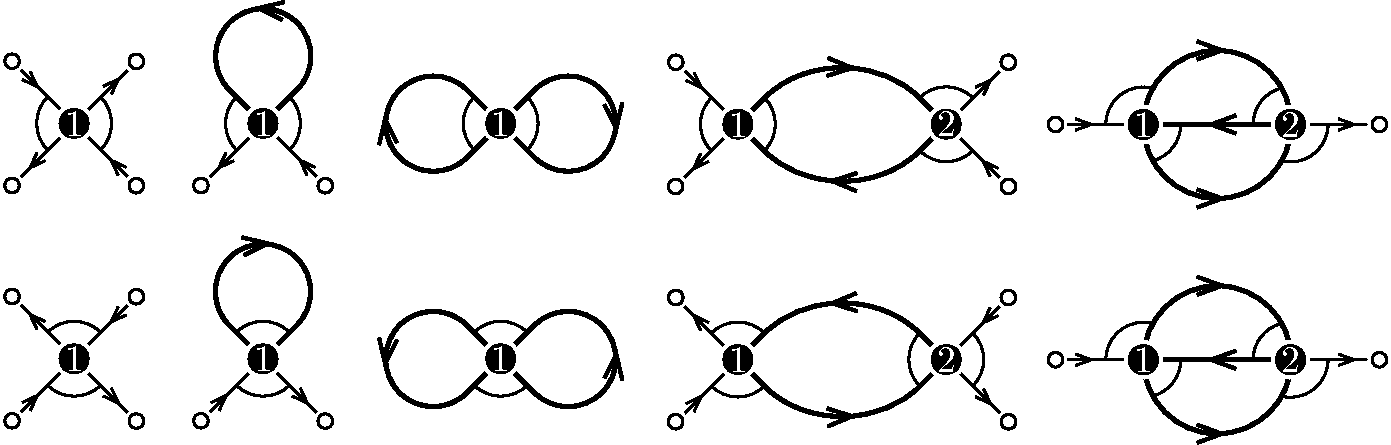
\includegraphics[scale=.6]{koszulQuivers}}
%%	\caption{The Koszul duals of the (blossoming) quivers of \fref{fig:quivers}.}
%%	\label{fig:koszulQuivers}
%%\end{figure}
%
%The following proposition appears in \cite[Proposition 1.25]{OpperPlamondonSchroll}.  

\begin{proposition}[{\cite[Prop.\,1.25]{OpperPlamondonSchroll}}]
\label{prop:dualityKoszul1}
Let~$\dissection$ and~$\dissection\dual$ be two dual cellular dissections of a marked surface~$(\surface, V\sqcup V\dual)$.
The bound quivers~$\bar Q_{\dissection}$ and~$\bar Q_{\dissection\dual}$ are Koszul dual to each other.
See \fref{fig:quiversDissections}.
\end{proposition}

%\begin{proof}
%The duality provides a bijection~$a\in (Q_\dissection)_0\mapsto a\dual\in (Q_{\dissection\dual})_0$, and also induces a bijection~${\alpha \in (Q_\dissection)_1 \mapsto \alpha\dual \in (Q_{\dissection\dual})_1}$ with~$s(\alpha\dual) = t(\alpha)\dual$ and~$t(\alpha\dual) = s(\alpha)\dual$.
%Moreover, for any two composable arrows~$\alpha,\beta\in(Q_\dissection)_0$, we have~$\alpha\beta\in I_\dissection$ if and only if~$s(\alpha),t(\alpha),t(\beta)$ are three consecutive edges of a~$\dissection$-cell~$f$, if and only if~$s(\alpha)\dual,t(\alpha)\dual,t(\beta)\dual$ are three consecutive edges in~$\dissection\dual$ ending in~$f\dual$, if and only if~$\beta\dual\alpha\dual\notin I_{\dissection\dual}$.
%\end{proof}

\subsection{The surface of a locally gentle bound quiver}
\label{subsec:Q2D}

We now associate a surface to a locally gentle bound quiver.
This construction yields the same surface as the one constructed in \cite{OpperPlamondonSchroll}. % (see Rem.\,\ref{rem:comparisonWithOPS} for a comparison).

\begin{definition}
\label{def:surfaceQuiver}
The surface~$\surface_{\bar Q}$ of a locally gentle bound quiver~$\bar Q = (Q,I)$ is the surface obtained from the blossoming quiver~$\bar Q\blossom$ as follows:
\begin{enumerate}[(i)]
\parpic(5cm,2cm)(-2pt, 115pt)[r][b]{\begin{tikzpicture}[
	scale=1.5,
	thick,
	decoration={markings, mark=at position 0.5 with {\arrow{>}}},
	roundNode/.style={circle, fill=black, inner sep=2pt, outer sep=1.5pt}
	]
	\node[roundNode, label={[label distance=-3pt]left:{$s(\alpha)$}}] (s) at (-1,0) {};
	\node[roundNode, label={[label distance=-3pt]right:{$t(\alpha)$}}] (t) at (1,0) {};
	\node[roundNode, fill=green, label={[label distance=-3pt]above:{$\green v(\alpha)$}}] (v) at (0,1) {};
	\node[roundNode, fill=red, label={[label distance=-3pt]below:{$\red f\dual(\alpha)$}}] (vd) at (0,-1) {};
	\draw[color=black, postaction={decorate}] (s) -> (t) node[midway, above] {$\alpha$};
	\pic [draw, angle radius=.7cm] {angle = s--t--vd};
	\pic [draw, angle radius=.7cm] {angle = vd--s--t};
	\draw[color=green, postaction={decorate}] (v) -> (s) node[midway, above left, outer sep=-3pt] {$\green \Enrs{\alpha}$};
	\draw[color=green, postaction={decorate}] (v) -> (t) node[midway, above right, outer sep=-3pt] {$\green \Enrt{\alpha}$};
	\draw[color=red, postaction={decorate}] (vd) -> (s) node[midway, below left, outer sep=-3pt] {$\red \Ers{\alpha}$};
	\draw[color=red, postaction={decorate}] (vd) -> (t) node[midway, below right, outer sep=-3pt] {$\red \Ert{\alpha}$};
\end{tikzpicture}
}
\item for each arrow~$\alpha \in Q_1\blossom$, consider a lozenge~$L(\alpha)$ with sides
%\begin{alignat*}{2}
\(
\begin{array}{llll}
\qquad & \Enrs{\alpha} = [v(\alpha), s(\alpha)] \quad & \Enrt{\alpha} = [v(\alpha), t(\alpha)] \quad & \text{(green)} \\
\qquad & \Ers{\alpha} = [f\dual(\alpha), s(\alpha)] \quad & \Ert{\alpha} = [f\dual(\alpha), t(\alpha)] \quad & \text{(red)}
\end{array}
\)
%\end{alignat*}

\item for any~$\alpha, \beta \in Q_1\blossom$ with~$t(\alpha) = s(\beta)$, identify:
    \begin{compactitem}
    \item $\Ert{\alpha}$ with~$\Ers{\beta}$ if~$\alpha\beta \in I$,
    \item $\Enrt{\alpha}$ with~$\Enrs{\beta}$ if~$\alpha\beta \notin I$.
    \end{compactitem}
\end{enumerate}
The orientations on the edges are only used for identifications and can be immediately forgotten.
\end{definition}

Def.\,\ref{def:surfaceQuiver} constructs an orientable surface~$\surface_{\bar Q}$ with boundaries.
\fref{fig:surfaces} illustrates this construction for the quivers of \fref{fig:quivers}.

\begin{figure}[h]
	\centerline{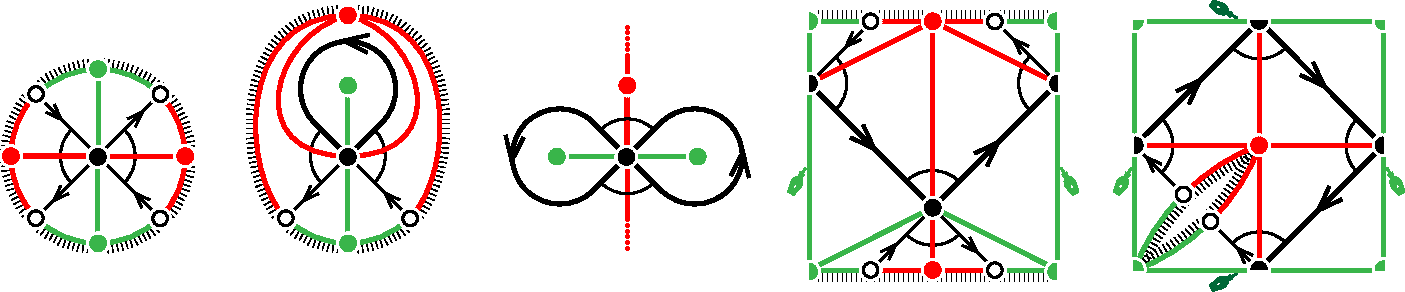
\includegraphics[scale=.7]{surfaces}}
	\caption{The surface~$\surface_{\bar Q}$ for the quivers~$\bar Q$ of \fref{fig:quivers}.}
	\label{fig:surfaces}
\end{figure}

%\begin{remark}
%We could equivalently construct the surface~$\surface_{\bar Q}$ as follows:
%\begin{itemize}
%\item consider one $(\ell+1)$-gon~$P_\omega$ for each straight walk~$\omega$ of length~$\ell$ in~$\bar Q$ or in~$\bar Q\koszul$ (just closing~$\omega$ with an additional edge connecting~$t(\omega)$ to~$s(\omega)$),
%\item for each arrow~$\alpha \in Q_1\blossom$, consider the only straight walks~$\omega$ of~$\bar Q$ and~$\omega\koszul$ of~$\bar Q\koszul$ containing~$\alpha$, and glue the polygons~$P_\omega$ and~$P_{\omega\koszul}$ along their edges corresponding to~$\alpha$.
%\end{itemize}
%\end{remark}
%
%The advantage of Definition~\ref{def:surfaceQuiver} is that it automatically endows~$\surface_{\bar Q}$ with two disjoint sets~$V_{\bar Q}$ and~${{V\dual}\!\!_{\bar Q}}$ of marked points and two dual cellular dissections~$\dissection_{\bar Q}$ and~${\dissection\dual\!\!_{\bar Q}}$ defined as follows.

\begin{definition}
\label{def:dissectionQuiver}
The surface~$\surface_{\bar Q}$ is endowed with
\begin{compactitem}
\item the set~$V_{\bar Q}$ of points~$v(\alpha)$ for~$\alpha \in Q_1\blossom$ after the identifications given by~(ii),
\item the $V_{\bar Q}$-dissection~$\dissection_{\bar Q}$ given by all sides~$\Enrs{\alpha}$ and~$\Enrt{\alpha}$ for~$\alpha \in Q_1\blossom$ after the identifications given by~(ii).
\end{compactitem}
The set~${{V\dual}\!\!_{\bar Q}}$ and the ${{V\dual}\!\!_{\bar Q}}$-dissection~${\dissection\dual\!\!_{\bar Q}}$ are defined similarly by using $f\dual(\alpha)$, $\Ers{\alpha}$ and $\Ert{\alpha}$.
\end{definition}

\begin{proposition}
\label{prop:dissectionsAreCellular}
Let~$\bar Q$ be a locally gentle bound quiver.
Then the dissections~$\dissection_{\bar Q}$ and~$\dissection\dual\!\!_{\bar Q}$ are cellular and dual to each other.
\end{proposition}

%\begin{proof}
%In the construction of~$\surface_{\bar Q}$, if two arrows~$\alpha$ and~$\beta$ of~$\bar Q \blossom$ are such that~${t(\alpha) = s(\beta)}$ and~${\alpha\beta \in I\blossom}$, then the vertices~$v(\alpha)$ and~$v(\beta)$ are identified on the surface.
%Thus, any two arrows of a given path contribute to the same vertex of~$V_{\bar Q}$, so~$V_{\bar Q}$ is in bijection with the set of maximal paths in~$\bar Q\blossom$.
%
%Let~$v\in V_{\bar Q}$. The situation around~$v$ is as follows, depending on whether~$v$ corresponds to a finite or infinite maximal path of~$\bar Q\blossom$:
%
%\begin{figure}[h]
%	\centerline{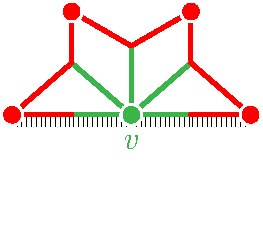
\includegraphics[scale=.7]{halfStar} \qquad 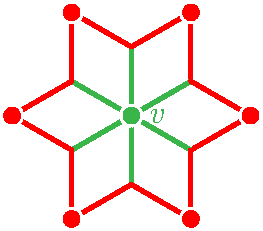
\includegraphics[scale=.7]{star}}
%	\caption{Two possible situations around~$v$: on the left,~$v$ corresponds to a finite maximal path of~$\bar Q$, while on the right,~$v$ corresponds to an infinite one.}
%	\label{fig:stars}
%\end{figure}
%
%In both cases, we see that~$v$ is enclosed in a polygon of~$\dissection_{\bar Q}\dual$.  This shows that~$\dissection_{\bar Q}\dual$ is a cellular dissection of~$\surface_{\bar Q}$.
%Dually, one shows that~$\dissection_{\bar Q}$ is also a cellular dissection.
%
%Moreover, by construction, each edge of~$\dissection_{\bar Q}$ which is not on the boundary of~$\surface_{\bar Q}$ crosses exactly one edge of~$\dissection_{\bar Q}\dual$, and vice versa.
%This shows that~$\dissection_{\bar Q}$ and~$\dissection_{\bar Q}\dual$ are dual to each other.
%\end{proof}

%The following statement immediately follows from the definitions and was probably already observed by the reader on \fref{fig:surfaces}.

\begin{theorem}
\label{thm:bijectionLocallyGentleAndSurfaces}
Up to isomorphism, the constructions of Defs.\,\ref{def:quiverDualDissections} \& \ref{def:surfaceQuiver} are inverse~to~each other.
They induce a bijection between the set of isomorphism classes of locally gentle bound quivers and the set of homeomorphism classes of marked surfaces with a pair of dual cellular dissections.
\end{theorem}

\begin{remark}
\label{rem:propertiesSurface}
The following observations are useful for the computation of examples.
\begin{compactenum}[(i)]
\item The set~$V_{\bar Q}$ has one vertex for each straight walk in~$\bar Q$ (equivalently, for each maximal path in~$\bar Q$).
      Finite straight walks yield vertices on the boundary of~$\surface_{\bar Q}$, while infinite cyclic straight walks in~$\bar Q$ yield punctures of~$\surface_{\bar Q}$ in~$V_{\bar Q}$.
      We denote by~$p$ the number of infinite cyclic straight walks in~$\bar Q$.
\item \label{item:edges}
      The dissection~$\dissection_{\bar Q}$ has one edge for each vertex~$a \in \bar Q_0$, obtained by concatenation of the sides~$\Enrt{\alpha} = \Enrs{\beta}$ and~$\Enrt{\alpha'} = \Enrs{\beta'}$ where~$a = t(\alpha) = s(\beta) = t(\alpha') = s(\beta')$, $\alpha\beta \notin I$ and~$\alpha'\beta' \notin I$. We denote by~$\edgeof(a)$ the edge of~$\dissection_{\bar Q}$ corresponding to~$a$.
\item The dissection~$\dissection_{\bar Q}$ has one $\ell$-cell for each straight walk of length~$\ell$ in~$\bar Q\koszul$.
\item Similar statements hold dually for~${{V\dual}\!\!_{\bar Q}}$ and~${\dissection\dual\!\!_{\bar Q}}$, and we define~$p\dual$ and~$\dualedgeof(a)$ similarly.
\item The number of punctures of~$\surface_{\bar Q}$ is the number~$p + p\dual$ of infinite straight walks in~$\bar Q$ and~$\bar Q\koszul$.
\item \label{item:boundary}
      The number~$b$ of boundary components of~$\surface_{\bar Q}$ can be computed as follows.
      There are two natural perfect matchings whose vertices are the blossom vertices of~$\bar Q$: one is obtained by joining the endpoints of each finite straight walk of~$\bar Q$, and the other is obtained similarly from~$\bar Q \koszul$.
      Let~$G$ be the superposition of these two perfect matchings.
      Then the number~$b$ of boundary components of~$\surface_{\bar Q}$ is the number of connected components of~$G$.
\item The genus of the surface~$\surface_{\bar Q}$ is
      \(
       g = (|Q_1| - |Q_0| - b - p - p\dual + 2)/2,
      \)
      where~$b$ is the number of boundary components (see above for a way to compute~$b$) and~$p + p\dual$ the number of punctures (\ie infinite straight walks in~$\bar Q$ and in~$\bar Q\koszul$).
%      Indeed, ${2g = 2-\chi(\surface_{\bar Q})}$, where~$\chi(\surface_{\bar Q})$ is the Euler characteristic of~$\surface_{\bar Q}$.
%      The dissection~$\dissection$ provides a cellular decomposition of~$\surface_{\bar Q}$ on which we fill the boundary components with disks.  
%      The number of faces of this cellular decomposition is~$b + p\dual$, its number of edges is~$|Q_0|$ and its number of vertices is the number of straight walks in~$\bar Q$, which is equal to~$2|Q_0| - |Q_1| + p$.
%      The above formula for~$g$ follows.
\end{compactenum}
\end{remark}

\begin{proposition}
\label{prop:dualityKoszul2}
For any gentle bound quiver~$\bar Q$ with Koszul dual~$\bar Q\koszul$, the surfaces~$\surface_{\bar Q}$ and~$\surface_{\bar Q\koszul}$ coincide, but~$\dissection_{\bar Q\koszul} = {\dissection\dual\!\!_{\bar Q}}$ and~${\dissection\dual\!\!_{\bar Q\koszul}} = \dissection_{\bar Q}$.
\end{proposition}

\begin{example}
\label{exm:cycle}
Consider the family of \defn{cycle quivers} indicated in \fref{fig:cyclesSurfaces}.
%Consider the family of \defn{cycle quivers} indicated in \fref{fig:cyclesQuivers}.
%%
%\begin{figure}[h]
%	\centerline{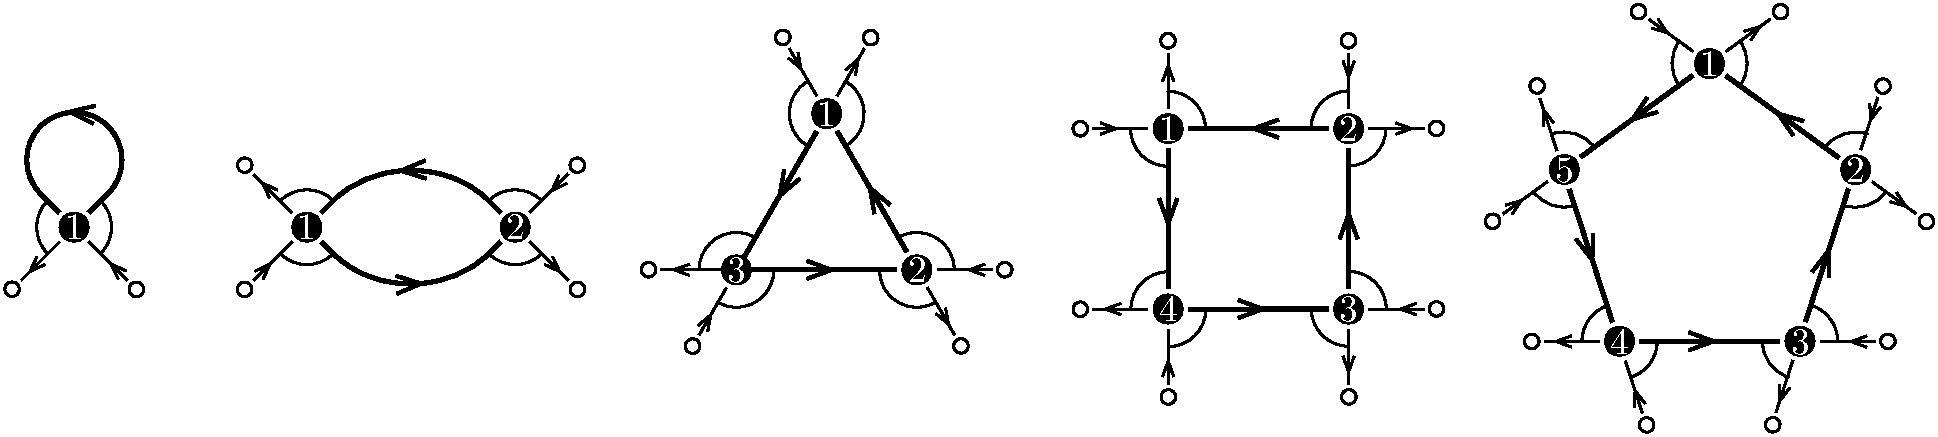
\includegraphics[scale=.45]{cyclesQuivers}}
%	\caption{The cycle quivers with~$1, 2, 3, 4, 5$ vertices.}
%	\label{fig:cyclesQuivers}
%\end{figure}
%%
We apply Rem.\,\ref{rem:propertiesSurface} to understand the corresponding surfaces.
The corresponding perfect matchings (see Rem.\,\ref{rem:propertiesSurface}\,\eqref{item:boundary}) form a cycle with green and red arrows alternating.
Moreover, $\bar Q$ has~$1$ infinite straight walk, while~$\bar Q\koszul$ has none.
Since~$|Q_1| = |Q_0|$, the corresponding surfaces are punctured disks ($1$ boundary component, $1$ puncture and genus~$0$).
See \fref{fig:cyclesSurfaces}.
%The first few corresponding surfaces are represented in \fref{fig:cyclesSurfaces} (see Figures~\ref{fig:surfaces} and~\ref{fig:reversedPathsSurfaces} for the cycles with $1$ or~$2$ vertices, recalling that~$\bar Q$ and~$\bar Q\koszul$ yield the same surface).

\begin{figure}[t]
	\centerline{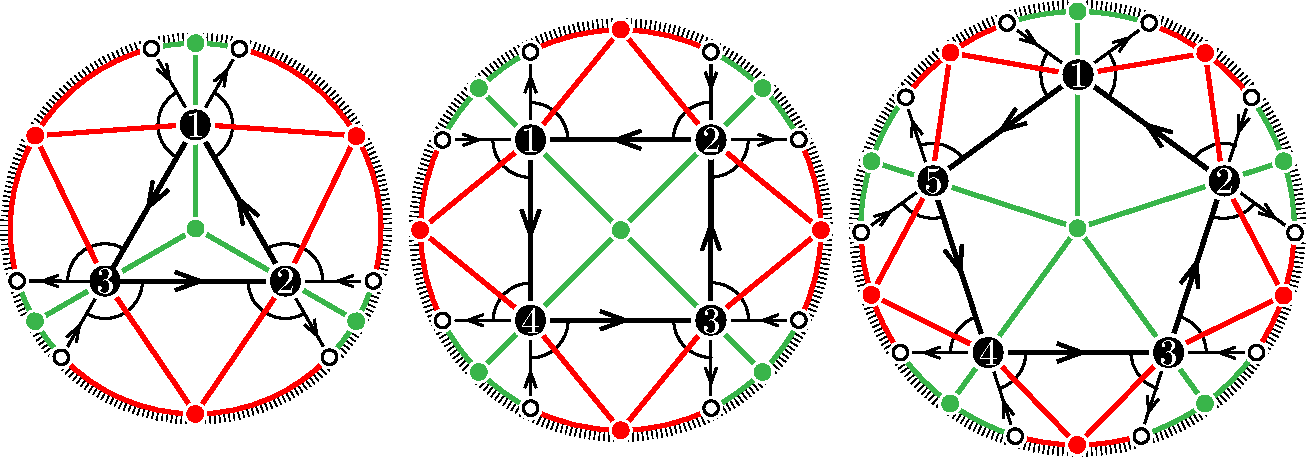
\includegraphics[scale=.7]{cyclesSurfacesBis}}
	\caption{The surface~$\surface_{\bar Q}$ for the cycle quivers with~$3, 4, 5$ vertices.}
	\label{fig:cyclesSurfaces}
\end{figure}
\end{example}

%\begin{remark}
%\label{rem:comparisonWithOPS}
%The construction of the surface given in Definition \ref{def:surfaceQuiver} yields the same surface as the one constructed in \cite{OpperPlamondonSchroll}.
%A notable difference is that in \cite{OpperPlamondonSchroll}, only~$\dissection_{\bar Q}$ is given, and~$\dissection\dual\!\!_{\bar Q}$ is deduced (it is called the dual lamination).
%Another minor difference is that the construction in \cite{OpperPlamondonSchroll} is written only for gentle algebras, while here it is generalized to locally gentle algebras.
%
%The major difference with \cite{OpperPlamondonSchroll} is the application of the surface of a (locally) gentle algebra: there, it is used as a model for the derived category of the gentle algebra (graded arcs correspond to indecomposable objects in that category), while here, it will be used as a model for walks in~$\bar Q$. % ($\dissection_{\bar Q}$-accordions will correspond to walks in~$\bar{Q}$, see Prop.\,\ref{prop:walks=arcs}).
%\end{remark}

\subsection{Non-crossing and non-kissing complexes coincide}

Let~$\bar Q$ be a locally gentle bound quiver.
For each edge of the dissection~$\dissection_{\bar Q}$ on~$\surface_{\bar Q}$, we fix a point on the interior of this edge, which we call its ``middle point'' (this is the black vertex on the pictures).
To each walk on~$\bar Q$, we will now associate a~$\dissection_{\bar Q}$-accordion.

\begin{definition}
\label{def:curveOfAnArrow}
For any arrow~$\alpha$ on $\bar Q\blossom$, let~$\curveof(\alpha)$ be the curve on~$\surface_{\bar Q}$ which goes from the middle point of the edge of~$\dissection$ corresponding to $s(\alpha)$ to the middle point of the edge of~$\dissection$ corresponding to $t(\alpha)$ by following the angle corresponding to~$\alpha$.
Define~$\curveof(\alpha^{-1})$ to be~$\curveof(\alpha)^{-1}$.
\end{definition}

\begin{definition}
\label{def:curveOfAWalk}
Let~$\omega = \prod_{i < \ell < j} \alpha_\ell^{\varepsilon_\ell}$ be a (possibly infinite) walk on~$\bar Q$. 
Define the curve~$\curveof(\omega)$ to be the concatenation of the curves~$\curveof(\alpha_\ell^{\varepsilon_\ell})$ of Def.\,\ref{def:curveOfAnArrow}.
\end{definition}

In practice, we will represent~$\curveof(\omega)$ by a curve which intersects itself only transversaly, and such that if it circles infinitely around a puncture, then it spirals towards it.

\begin{lemma}
\label{lemm:curveOfAWalkIsAccordion}
Let~$\omega$ be a walk on~$\bar Q$.  Then~$\curveof(\omega)$ is a~$\dissection_{\bar Q}$-accordion.
\end{lemma}

%\begin{proof}
%This is because~$\curveof(\omega)$ follows angles in~$\dissection_{\bar Q}$ by definition.
%\end{proof}

\begin{lemma}
\label{lemm:accordionsAreCurvesOfWalks}
Let~$\gamma$ be a~$\dissection_{\bar Q}$-accordion.  There exists a unique undirected walk~$\walk(\gamma)$ such that we have~$\curveof(\walk(\gamma)) = \gamma$.
\end{lemma}

%\begin{proof}
%We can assume that~$\gamma$ intersects itself and the edges of~$\dissection_{\bar Q}$ transversaly and minimally, in the sense that~$\gamma$ does not cross an edge twice in succession in opposite directions (see Definition~\ref{def:crossingCurves}).
%Then~$\gamma$ is completely determined by its sequence of intersection points with the edges of~$\dissection_{\bar Q}$, since the dissection is cellular.
%Two successive intersection points in this sequence define an angle between two edges of~$\dissection_{\bar Q}$, which corresponds to an arrow in~$\bar Q$.
%Thus the sequence of intersection points defines a walk~$\walk(\gamma)$ on~$\bar Q$.
%By construction, we have that~$\curveof(\walk(\gamma)) = \gamma$.
%Is also follows from the construction above and from Definition~\ref{def:curveOfAWalk} that~$\walk(\curveof(\omega)) = \omega$ for any walk~$\omega$.
%This finishes the proof.
%\end{proof}
%
%The above implies the following.

\begin{proposition}
\label{prop:walks=arcs}
The maps~$\curveof(-)$ and~$\walk(-)$ induce mutually inverse bijections between the set of undirected walks on~$\bar Q$ and the set of~$\dissection_{\bar Q}$-accordions on~$\surface_{\bar Q}$.
\end{proposition}

\begin{lemma}
\label{lem:nonKissing=nonCrossing}
Two undirected walks~$\omega_1$ and~$\omega_2$ on~$\bar Q$ are non-kissing if and only if the corresponding $\dissection_{\bar Q}$-accordions~$\curveof(\omega_1)$ and~$\curveof(\omega_2)$ are non-crossing on~$\surface_{\bar Q}$.
\end{lemma}

%\begin{proof}
%A kiss between two walks~$\omega$ and~$\omega'$ is depicted on \fref{fig:kissings}.
%
%\begin{figure}[h]
%	\capstart
%	\centerline{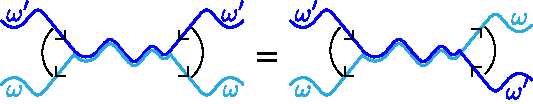
\includegraphics[scale=1]{kissings}}
%	\caption{Two representations of a pair of kissing walks.}
%	\label{fig:kissings}
%\end{figure}
%The left hand side of the picture is as in \fref{fig:kissing}, and the right hand side is simply a different representation of it.
%On the surface~$\surface_{\bar Q}$, the dual dissections~$\dissection$ and~$\dissection\dual$ are as on \fref{fig:kissingVSCrossing} (right).
%
%\begin{figure}[h]
%	\capstart
%	\centerline{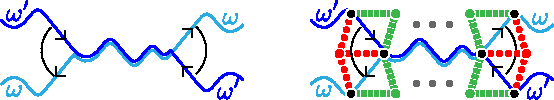
\includegraphics[scale=1]{kissingVSCrossing}}
%	\caption{Kissing walks on the quiver~$\bar Q$ correspond to crossing curves on the surface~$\surface_{\bar Q}$.}
%	\label{fig:kissingVSCrossing}
%\end{figure}
%
%The curves~$\curveof(\omega)$ and~$\curveof(\omega')$ on the surface follow~$\omega$ and~$\omega'$ on the picture.
%It is then clear that~$\omega$ and~$\omega'$ kiss if and only if~$\curveof(\omega)$ and~$\curveof(\omega')$ cross. 
%\end{proof}

\begin{theorem}
\label{thm:complexesCoincide}
The non-kissing complex and the non-crossing complex are isomorphic.
%The non-kissing complex~$\NKC$ and the non-crossing complex~$\NCC[\dissection_{\bar Q}, {\dissection\dual\!\!_{\bar Q}}]$ are isomorphic.
%\begin{compactitem}
%\item for any locally gentle bound quiver~$\bar Q$, the non-kissing complex~$\NKC$ is isomorphic to the non-crossing complex~$\NCC[\dissection_{\bar Q}, {\dissection\dual\!\!_{\bar Q}}]$,
%\item for any pair of dual cellular dissections~$\dissection, \dissection\dual$ of an oriented surface, the non-crossing complex~$\NCC$ is isomorphic to the non-kissing complex~$\NKC[\bar Q_{\dissection, \dissection\dual}]$.
%\end{compactitem}
\end{theorem}

%\begin{proof}
%The first point is a consequence of Proposition \ref{prop:walks=arcs}, Lemma \ref{lem:nonKissing=nonCrossing} and Proposition \ref{prop:accordionsSlaloms}.
%The second point is a consequence of Theorem \ref{thm:bijectionLocallyGentleAndSurfaces} and of the first point.
%\end{proof}

%\begin{remark}
%Note that our construction of the surface~$\surface_{\bar Q}$ implies that the quiver~$\bar Q$ is naturally embedded on~$\surface_{\bar Q}$.
%If we force all $\dissection$-accordions (or $\dissection\dual$-slaloms) to follow the arrows of~$\bar Q$, then a $\dissection$-accordion (or $\dissection\dual$-slalom) is really seen as a walk on~$\bar Q$.
%\end{remark}

%\newpage
%% if you use biblatex then this generates the bibliography
%% if you use some other method then remove this and do it your own way
\printbibliography



\end{document}
